\documentclass{beamer}

\mode<presentation> {
    \usetheme{Madrid}
}

\usepackage{graphicx}
\usepackage{booktabs}

\graphicspath{{../fig/}}

\title[Iterative Hessian Sketch]{Iterative Hessian Sketch for Constrained Least-Squares} 

\author{Lydia Hsu, Shuaiwen Wang} 

\date{\today} % Date, can be changed to a custom date

\begin{document}

\begin{frame}
    \titlepage
    
    \tiny Paper: \textit{Iterative Hessian Sketch: Fast and Accurate Solution Approximation
    for Constrained Least-Squares}
\end{frame}

\begin{frame}
    \frametitle{Problem description}

    \begin{itemize}
        \item<1-> Consider the \textbf{constrained least-squares}
            \begin{equation*}
                x_{ls} := \arg\min_{x \in C} \; \frac{1}{2} \|Ax-y\|^2_2
            \end{equation*}
            where \quad $C$: constraint; \quad $A \in \mathbb{R}^{n \times p}$: design matrix; \quad $y$: response.
        
        \item<2-> Issue: when $n$ large, computationally \textbf{expensive};
        \item<3-> Idea: ``sketch'' $A$ using $SA$;
        \item<4-> $S \in \mathbb{R}^{m \times n}$: sketching matrix; \quad
            $\mathbb{E} S^\top S = I_n$.
    \end{itemize}
\end{frame}

\begin{frame}
    \frametitle{Common sketching matrices}

    \begin{itemize}
        \item<1-> sub-Gaussian: $S_{ij} \sim_{iid} \frac{1}{\sqrt{m}}
            \mathcal{N}(0, 1)$; 
        \item<2-> random row sampling: randomly select $m$ rows from $I_n$
            (rescaled by $\sqrt{\frac{n}{m}}$);
        \item<3-> randomized orthogonal system: randomly select $m$ rows from
            an orthogonal matrix $H$ (rescaled by $\sqrt{\frac{n}{m}}$);
    \end{itemize}
\end{frame}

\begin{frame}
    \frametitle{Classical Sketch}
    
    \begin{itemize}
        \item<1-> Sketch not only $A$, but also $y$:
            \begin{equation*}
                x_{cs} := \arg\min_{x \in C} \; \frac{1}{2} \|SAx-Sy\|^2_2
           \end{equation*}
       \item<2-> Classical sketch is \textbf{sub-optimal}:
           assume a linear ground truth $y = Ax_* + w$:
           \begin{equation*}
               \|x_{cs} - x_*\| \sim \|x_{ls} - x_*\|
               \quad \Rightarrow \quad
               m = \Theta(n)
           \end{equation*}
       \item<3-> We expect the optimal method satisfies $m \approx O(p)$
           \textcolor{red}{Think about this part more carefully?};
    \end{itemize}

\end{frame}

\begin{frame}
    \frametitle{Hessian Sketch}
    \begin{itemize}
        \item<1-> Only sketch $A$, but not $y$:
            \begin{equation*}
                x_{hs} := \arg\min_{x\in C} \; \frac{1}{2} \| S Ax\|^2_2 - \langle A^\top y, x \rangle.
            \end{equation*}
        \item<2-> \textbf{Sub-optimal} in the same sense;
        \item<3-> With $m \sim O(p)$ sample size, we can obtain a weak result:
            \begin{equation*}
                \| x_{hs} - x_{ls} \| \leq \rho \|x_{ls}\|,
                \quad \text{w.h.p.}
            \end{equation*}
            where $\rho \in (0, \frac{1}{2})$.
        \item<4-> \textit{An iterative idea for improvement}: ``$\| x^{t+1} - x_{ls} \| \leq
            \rho \|x^{t} - x_{ls}\|$''?
    \end{itemize}
\end{frame}

\begin{frame}
    \frametitle{Iterative Hessian Sketch}

    A detailed idea:
    \begin{itemize}
        \item<1-> Given $x^t$, a modified least square with $x_{ls} -
            x^t$ as minimizer:
            \begin{equation*}
                \only<1>{\min_{u} \frac{1}{2} \| A(u + x^t) \|_2^2 - \langle A^\top y,
                (u + x^t) \rangle}
                \only<2->{\min_{u} \frac{1}{2} \| Au \|_2^2 - \langle A^\top (y -
                Ax^t), u \rangle}
            \end{equation*}
        \item<3-> The corresponding Hessian sketch:
            \begin{equation*}
                u^{t+1} = \arg\min_{u} \frac{1}{2} \| SAu \|_2^2 - \langle A^\top (y - Ax^t), u \rangle
            \end{equation*}
        \item<4-> Property of Hessian sketch: $\|u^{t+1} - (x_{ls} - x^t)\|
            \leq \rho \|x_{ls} - x^t\|$;
        \item<5-> Define $x^{t+1} = x^t + u^{t+1}$, then:
            \begin{equation*}
                \|x^{t+1} - x_{ls}\| \leq \rho \|x^t - x_{ls}\|,
                \quad \text{w.h.p.}
            \end{equation*}
 
    \end{itemize}
\end{frame}

\begin{frame}
    \frametitle{Iterative Hessian Sketch}
    \begin{block}{Algorithm}
        \begin{enumerate}
            \item Initialize $x^0 = 0$.\\
            \item For $t=1,...N$, generate independent sketches $S^t \in
                \mathbb{R}^{m \times n}$ and
                \begin{equation*}
                    x^t = \arg\min_{x \in C} \; \frac{1}{2} \| S^t A(x -
                    x^{t-1})\|^2_2 - \langle A^T(y-A x^{t-1}), x - x^{t-1} \rangle
                \end{equation*}
            \item Return $\hat{x} = x^N$.  
        \end{enumerate}
    \end{block}
\end{frame}

\begin{frame}
    \frametitle{Iterative Hessian Sketch}

    Properties of IHS:
    \begin{itemize}
        \item<1-> $m = O(p)$ to guarantee $\|x^t - x_{ls}\| \leq \rho
            \|x^{t-1} - x_{ls}\|$ in each iteration;
        \item<2-> To achieve an accuracy of $\epsilon$, we need
            $\log(\frac{1}{\epsilon})$ iterations;
        \item<3-> Optimality:
            \begin{itemize}
                \item<3-> To achieve the same bound as $\|x_{ls} - x_*\|\approx
                    O(\frac{1}{\sqrt{n}})$, we need $N=log(n)$ iterations;
                \item<4-> Union bound: $\|x^N - x_{ls}\| \leq
                    \rho^N \|x_{ls}\|$, \textit{w.h.p.}.
            \end{itemize}
    \end{itemize}
\end{frame}

\begin{frame}
    \frametitle{Simulations in the paper}
    \begin{figure}
        \begin{center}
            \begin{tabular}{ll}
                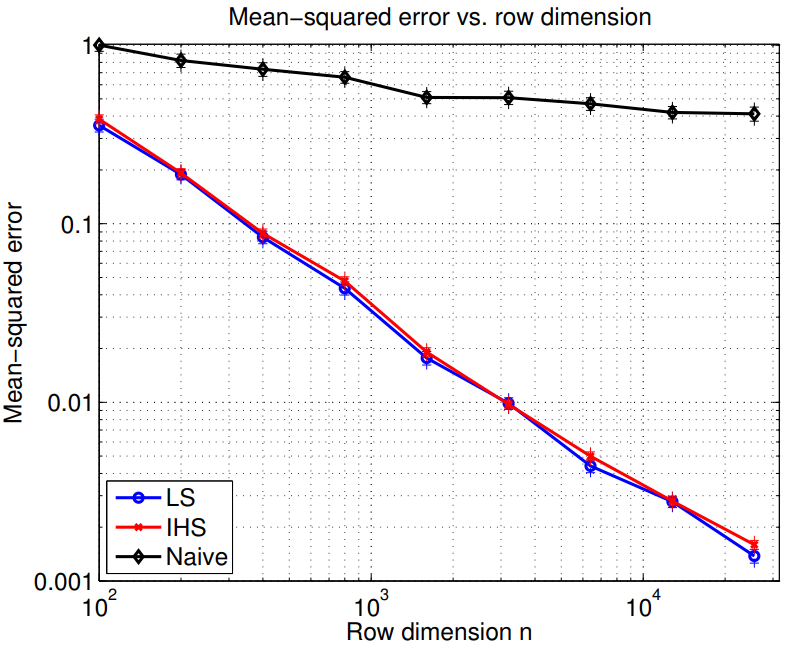
\includegraphics[scale=0.22]{ihs_paper_mse_vs_n_ihs_naive_compare.png}
                &
                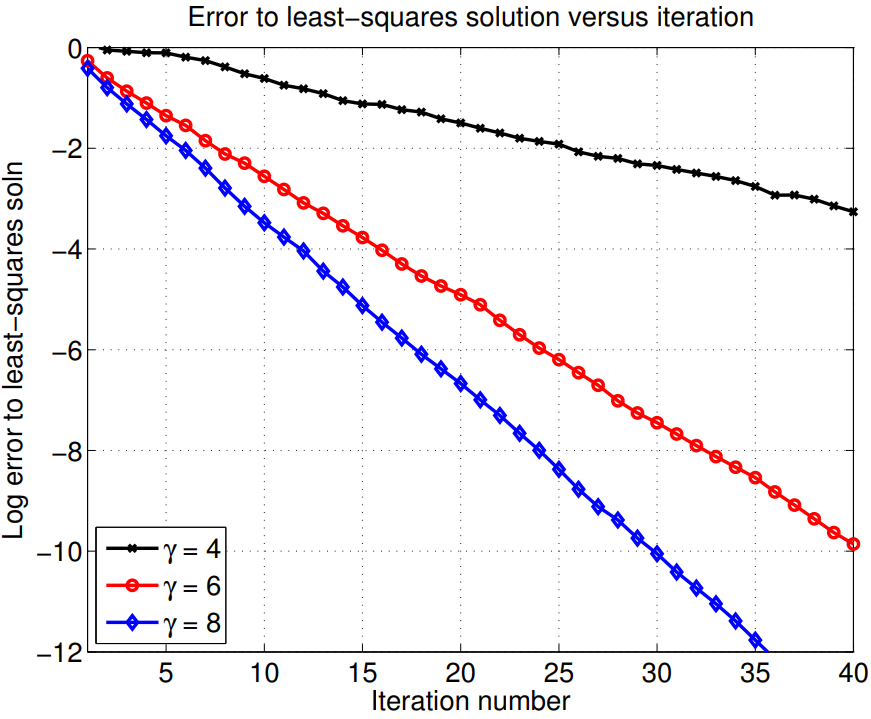
\includegraphics[scale=0.20]{ihs_paper_mse_vs_iter_ihs_diff_m.png}
            \end{tabular}
            \caption{Left: classical sketch vs. iterative hessian sketch;
            Right: different choices of $m=\gamma p$.}
        \end{center}
    \end{figure}
\end{frame}

\begin{frame}
    \frametitle{Simulations - different sketch matrices}
    \begin{figure}
        \begin{center}
            \begin{tabular}{ll}
                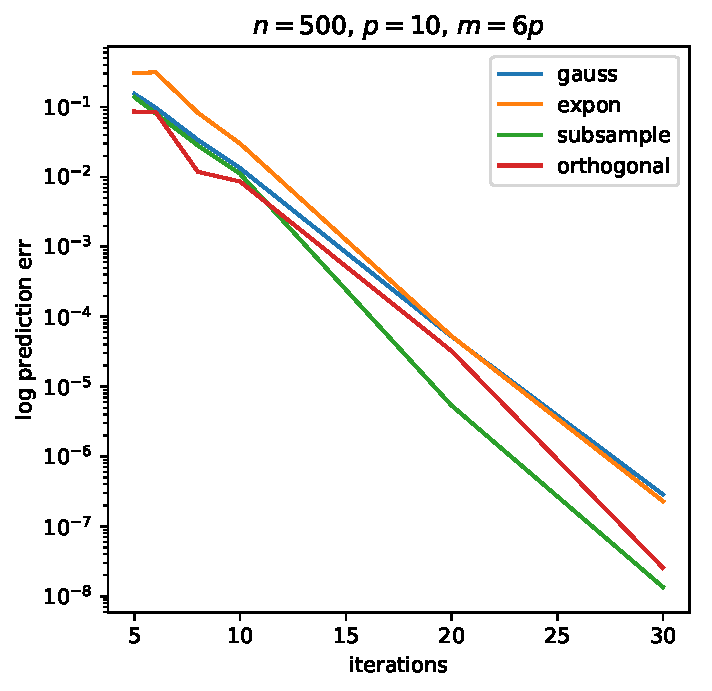
\includegraphics[scale=0.32]{diff_sketch_mat_err_vs_iter_n500_p10_m60.pdf}
                &
                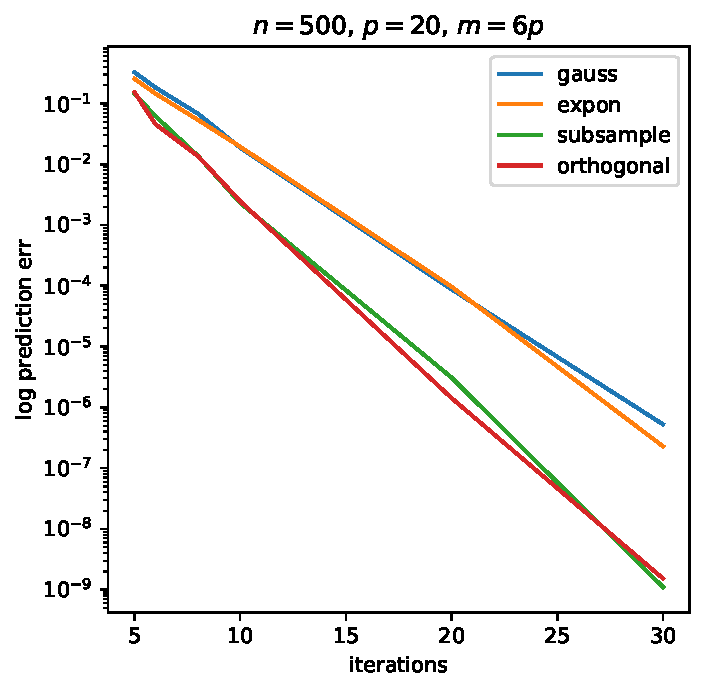
\includegraphics[scale=0.32]{diff_sketch_mat_err_vs_iter_n500_p20_m120.pdf}
            \end{tabular}
            \caption{Using different sketch matrices, under Gaussian design. ``expon'' means
            Laplace design.}
        \end{center}
    \end{figure}
\end{frame}

\begin{frame}
    \frametitle{Simulations - model mis-specifications}

    \begin{figure}
        \begin{center}
            \begin{tabular}{ll}
                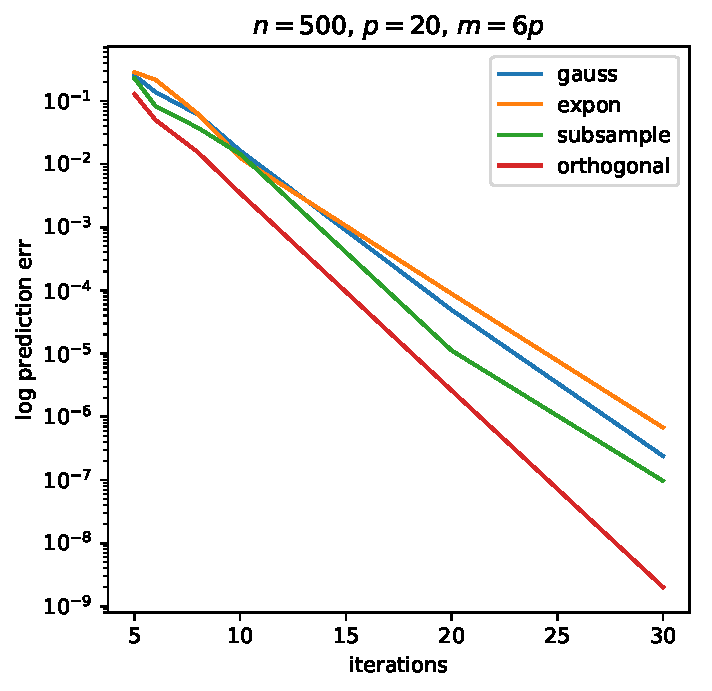
\includegraphics[scale=0.32]{exp_design_err_vs_iter_n500_p20_m120.pdf}
                &
                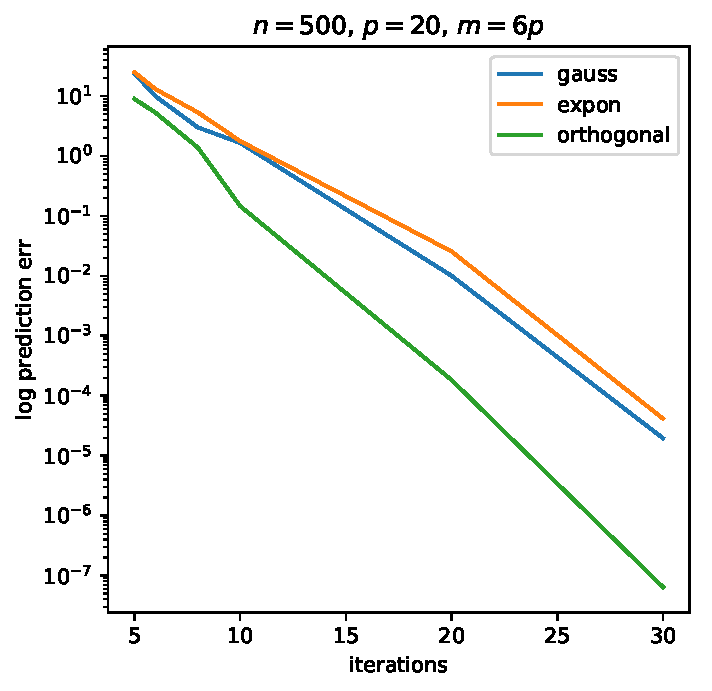
\includegraphics[scale=0.32]{cauchy_design_err_vs_iter_n500_p20_m120.pdf}
            \end{tabular}
            \caption{Left: exponential design; Right: Laplace design.}
        \end{center}
    \end{figure}
\end{frame}

\begin{frame}
    \frametitle{Simulations - model mis-specifications cont.}

    \begin{figure}
        \begin{center}
            \begin{tabular}{ll}
                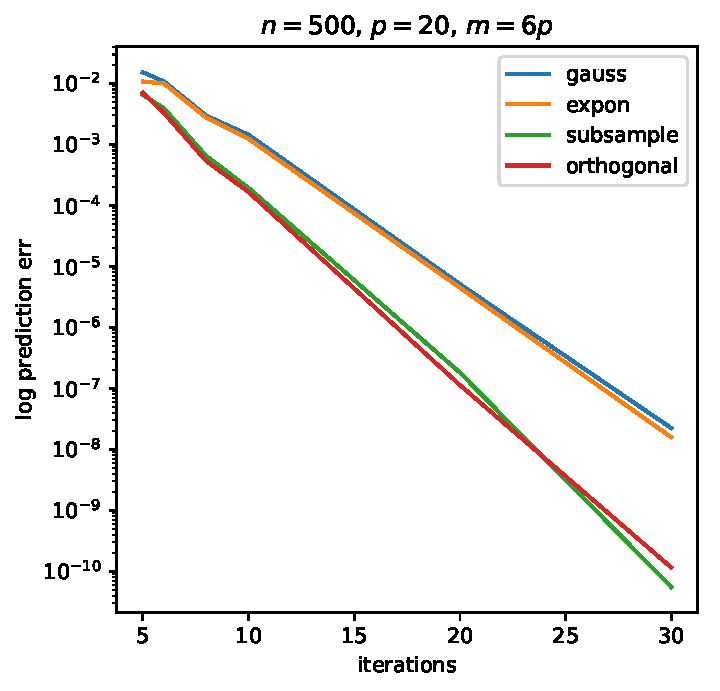
\includegraphics[scale=0.32]{sin_transform_err_vs_iter_n500_p20_m120.pdf}
                &
                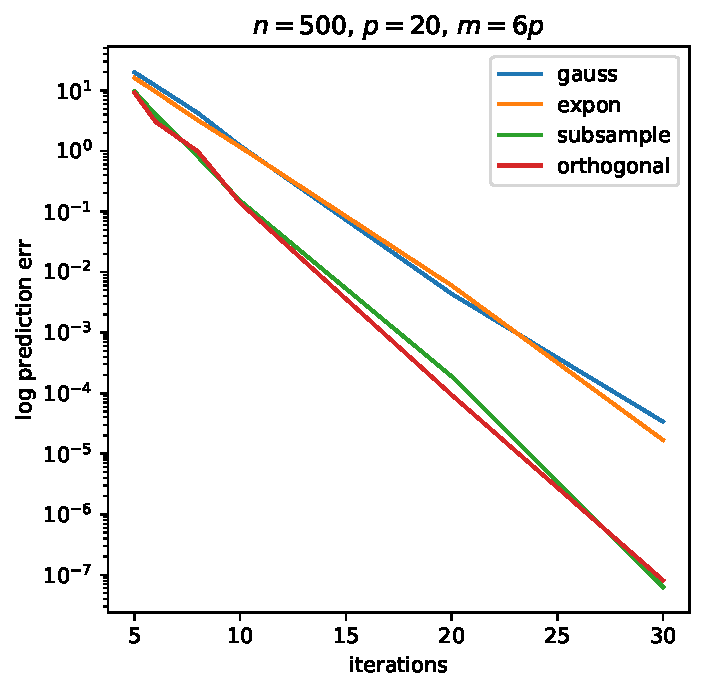
\includegraphics[scale=0.32]{cubic_transform_err_vs_iter_n500_p20_m120.pdf}
            \end{tabular}
            \caption{Left: $y=\sin(Ax) + w$; Right: $y=(Ax)^3 + w$. Both
            under Gaussian design. Large noise $w$ behabves similarly.}
        \end{center}
    \end{figure}
\end{frame}

\begin{frame}
    \begin{center}
        \Large Thank you!
    \end{center}
\end{frame}

\begin{frame}
    \frametitle{Evaluation for Sketch Performance}
    \begin{block}{Cost Approximation}
        In terms of $f$-cost, the approximated $\tilde{x}$ is said to be $\epsilon$-optimal if \\
        \vspace{.5cm}
        $f(x^{LS}) \leq f(\tilde{x}) \leq (1+\epsilon)^2 f(x^{LS})$.
    \end{block}
    
    \begin{block}{Solution Approximation}
        In terms of $f$-cost, the prediction norm defined as \\
        \vspace{.5cm}
        $\|\tilde{x} - x^{LS}\|_A := \frac{1}{\sqrt{n}} \|A(\tilde{x} - x^{LS})\|_2$.
    \end{block}
\end{frame}


\end{document}
